\documentclass[a4paper, 11pt]{report}
\usepackage{graphicx}
\usepackage{listings} 
\usepackage{subcaption}
\begin{document}

\section{parallel computing}
	\subsection{What is parallel computing}
The problem when facing large calculations is that they require a lot of computing power and thus time. Performing these calculations can be done with two types of computation, serial and parallel computing. Serial computing means, you have one compute unit (e.g. a single core CPU) available that performs all instructions on a certain set of data. This set of data will be broken into multiple smaller subparts that will be solved by a certain instruction. The single compute unit performs the instruction on every subpart in order to solve the whole part as shown in figure \ref{fig:SerialC}.
	\begin{figure}[ht]
		\centering
		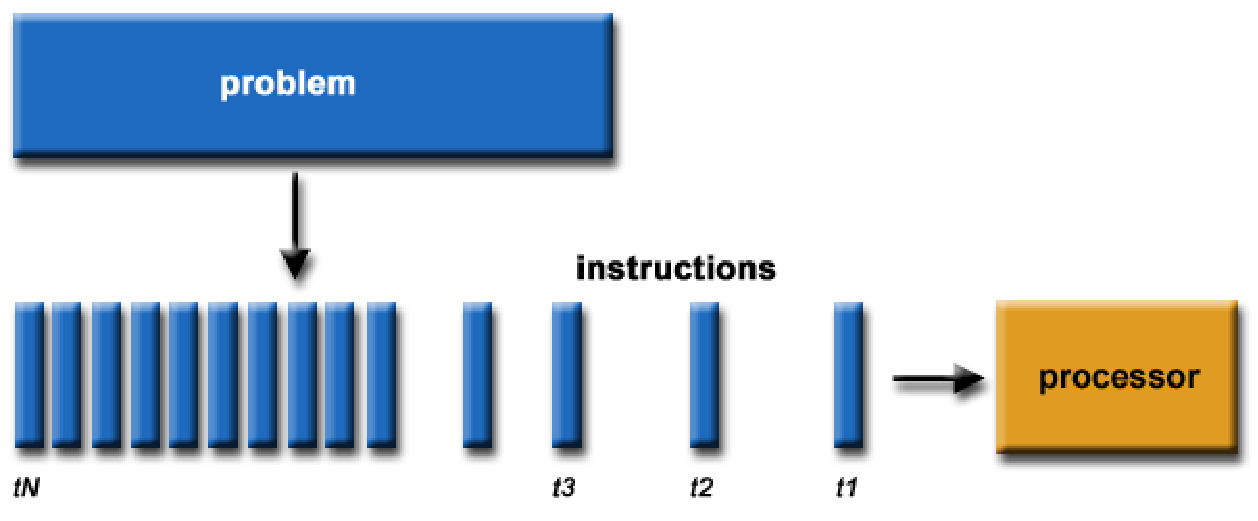
\includegraphics[scale=.4]{images/serialProblem.pdf}
		\caption{Workflow serial computing}
		\label{fig:SerialC}
	\end{figure}

Parallel computing, on the other hand, is the simultaneous use of multiple compute units, or a compute resource, to solve a computational problem. This compute resource can be a CPU with multiple cores, a combination of a CPU with different compute accelorators such as a GPU or even a whole network of computers and servers. We break apart the main problem in smaller subproblems as we did with serial computing. Now, since there are multiple compute units, we can distribute the subproblems among all these compute units. Every unit can now perform an instruction on their given subproblem simultaneously as shown in figure \ref{fig:ParallelC}.
	\begin{figure}[ht]
		\centering
		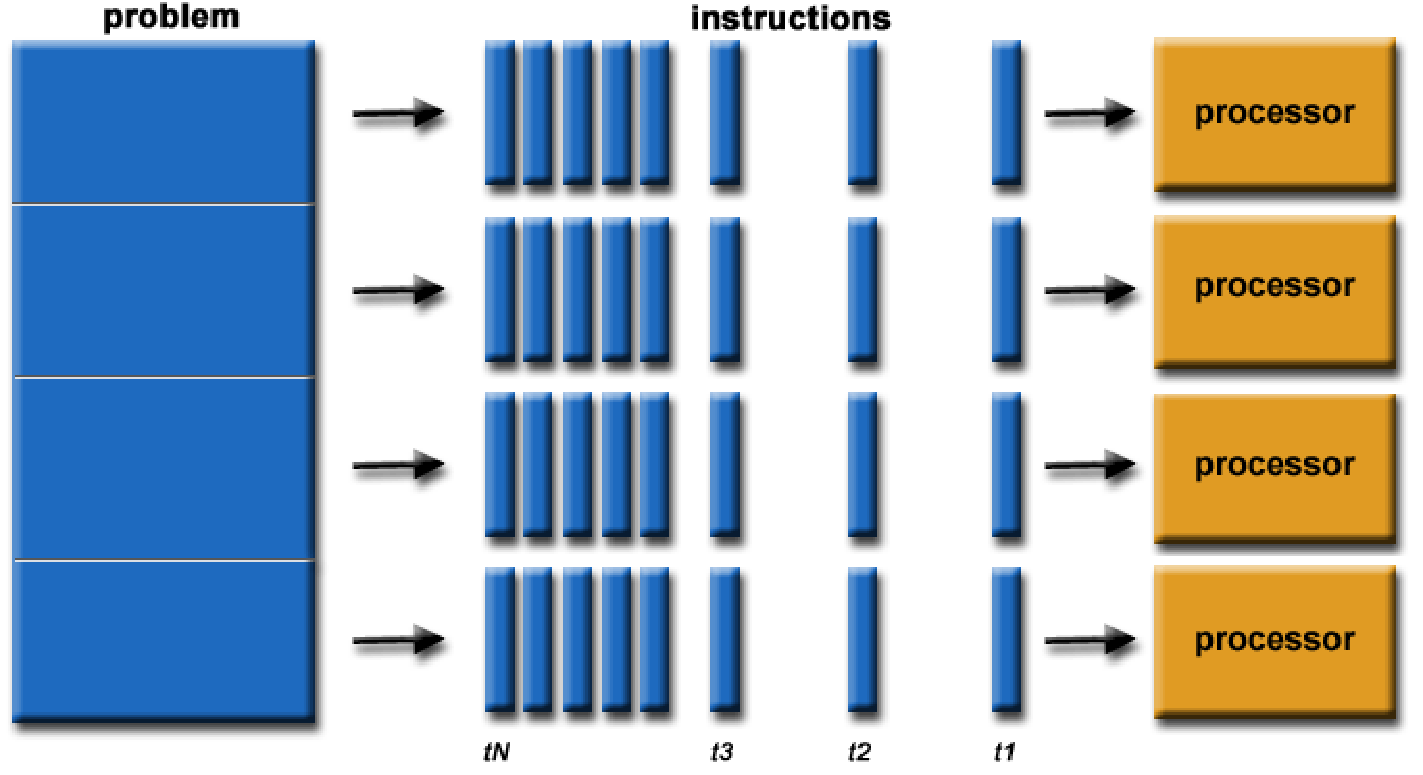
\includegraphics[scale=.4]{images/parallelProblem.pdf}
		\caption{Workflow parallel computing}
		\label{fig:ParallelC}
	\end{figure}
With multiple compute units executing one task, we will shorten the completion time and even have a potential cost saving. It also allows us to solve larger/complex problems since a single computer could suffer from limited memory. And last, we are able to access non-local resources in a network that would not be accessible from a local computer.

It is easy to conclude that the concept of parallel computing was to have a more efficient way to handle large sets of data such as huge databases, images or simulations that involve multiple parameters. It is also easier to handle complex data for example in algorithms \cite{barney2012parallel}.

	\subsection{Classification of parallel computing}
Parallel computing systems can be separated into different classes. According to Flynn's taxonomy, we can roughly place any of these systems in one of the four classes he defined. This classification was first studied and proposed by Michael Flynn in 1972 \cite{Unit2COPC}. The classifications are determined by two factors: instruction stream and data stream which both have two possible states being single or multiple. Figure \ref{fig:flynnTaxonomy} represents a the four possible classes from the Flynn's taxonomy \cite{barney2012parallel}.

	\begin{figure}[ht]
		\centering
		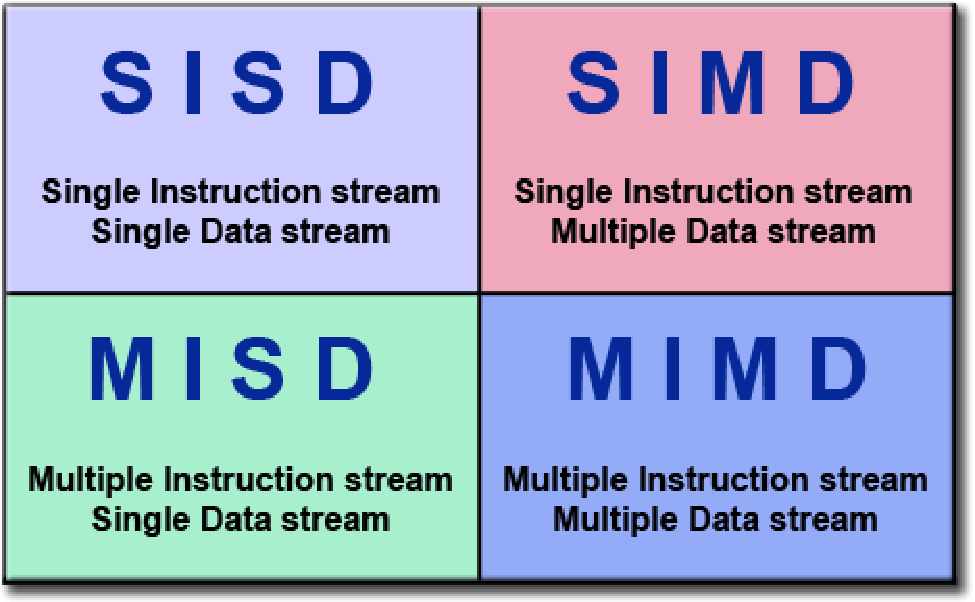
\includegraphics[scale=.5]{images/flynnsTaxonomy.pdf}
		\caption{Four possible classifications according to Flynn's Taxonomy}
		\label{fig:flynnTaxonomy}
	\end{figure}
	
	\begin{itemize}
		\item SISD
	\end{itemize}
The SISD class will have a single core processor executing a single data stream to operate on data stored in a single memory (figure \ref{fig:sisd}). This means that a parallel compute system cannot be classified as an SISD system, but Flynn's taxonomy was not made for just classifying parallel compute systems. Any traditional single-core processor falls into this category but it is usually old computers or older compute units that can be classified as SISD.
	
	\begin{itemize}
		\item SIMD
	\end{itemize}
Data is distributed amongst multiple processors who all execute the same instruction on this data (figure \ref{fig:simd}). Since we have access to multiple compute units, parallel computing can be categorized in this class. Furthermore, this is the class where we can categorize our subject of the thesis in since we have a large set of data divided over multiple data streams (MD) and only one instruction stream (SI) since all processing units will perform the same instruction on the data. The SIMD class contains the most modern computers, particularly those with a graphics processor unit (GPU).

	\begin{itemize}
		\item MISD
	\end{itemize}
Each processing unit operates on the data independently via separate instruction streams while a single data stream is fed into multiple processing untis (figure \ref{fig:misd}). This class knows very few applications. An example of an application is the use of multiple cryptography algorithms attempting to crack a single coded message.
	
	\begin{itemize}
		\item MIMD
	\end{itemize}
This time every processing unit is able to execute a different instruction stream on a different data stream (figure \ref{fig:mimd}). This means that any instruction can be applied on any data package for every compute unit. Most supercomputers, networked parallel computer clusters and "grids" can be classified as a MIMD compute system. Also, many MIMD architectures include SIMD execution sub-components.

\begin{figure}[ht]
	\centering
	\begin{subfigure}[t]{0.4\textwidth}
		\centering
		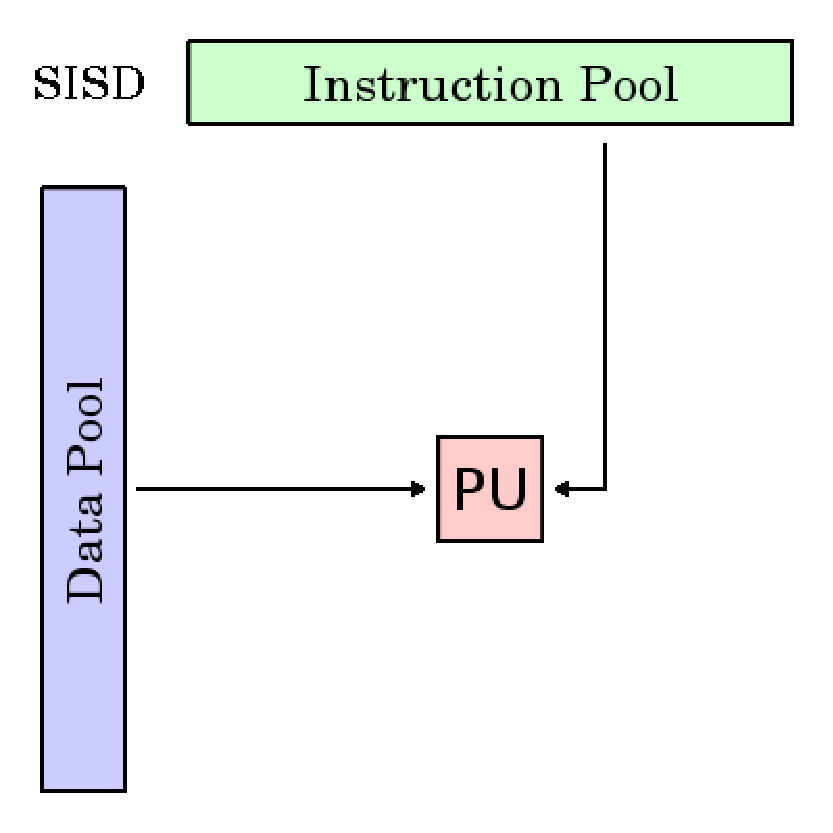
\includegraphics[scale=.3]{images/sisd.pdf}
		\caption{SISD}\label{fig:sisd}
	\end{subfigure}
	\begin{subfigure}[t]{0.4\textwidth}
		\centering
		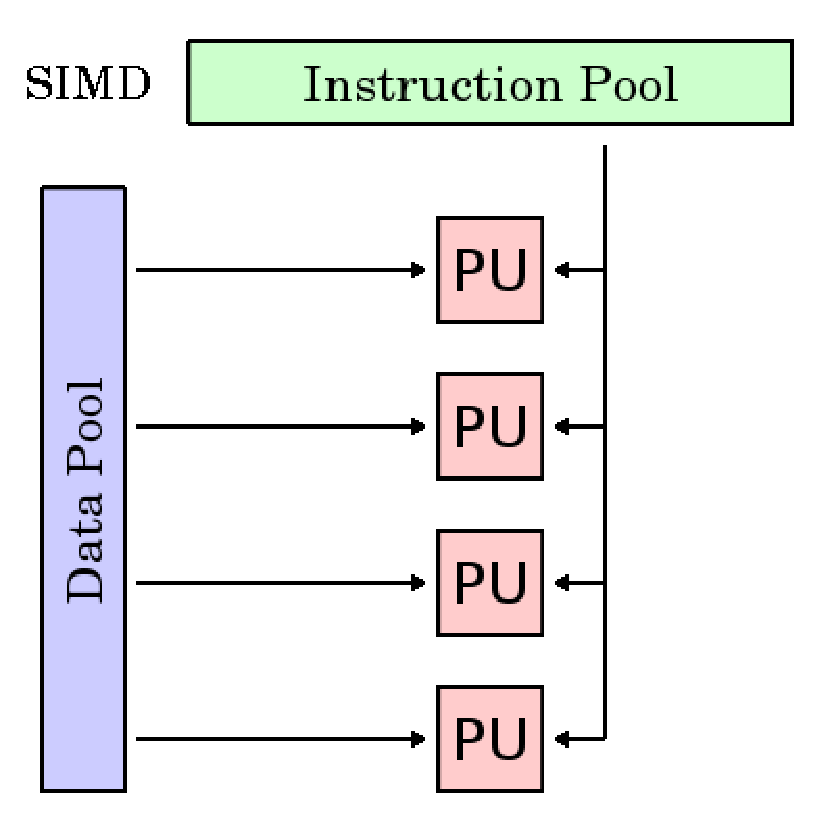
\includegraphics[scale=.3]{images/simd.pdf}
		\caption{SIMD}\label{fig:simd}
	\end{subfigure}
	\begin{subfigure}[t]{0.4\textwidth}
		\centering
		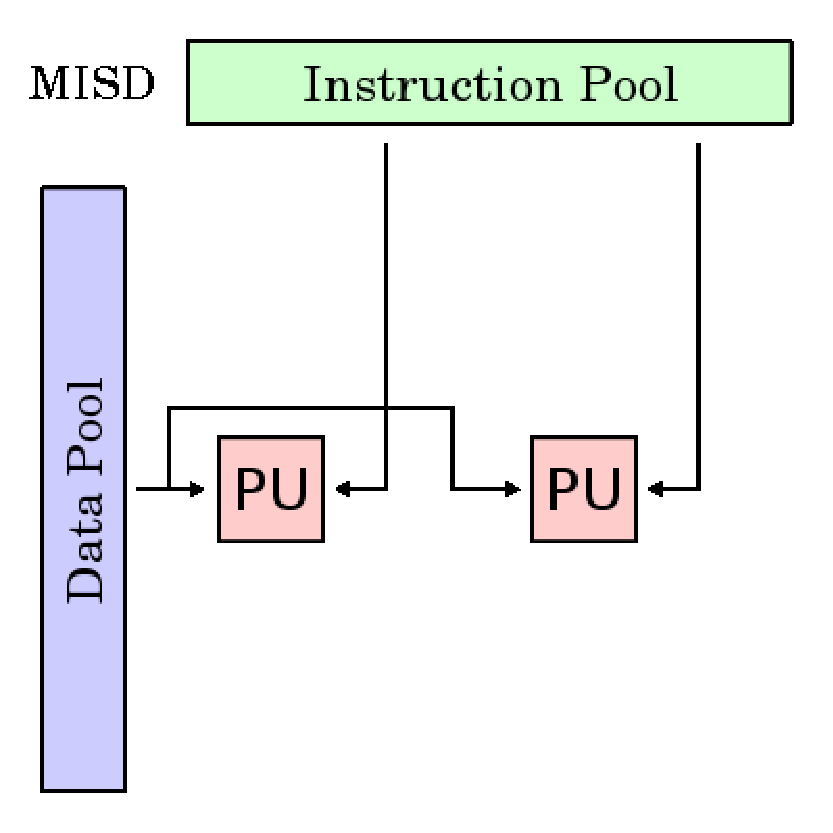
\includegraphics[scale=.3]{images/misd.pdf}
		\caption{MISD}\label{fig:misd}
	\end{subfigure}
	\begin{subfigure}[t]{0.4\textwidth}
		\centering
		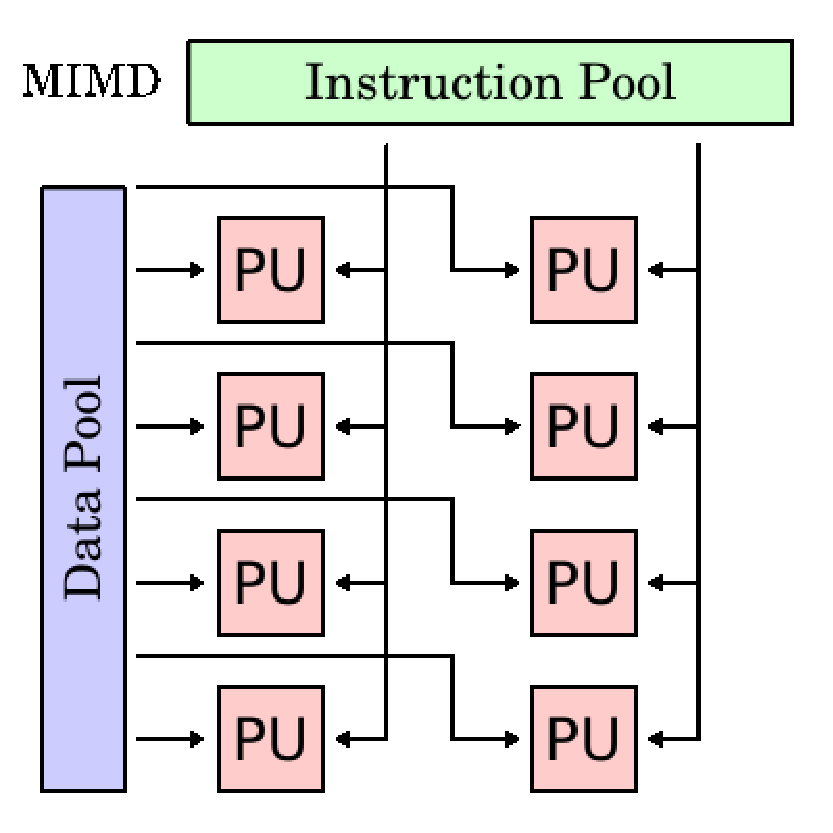
\includegraphics[scale=.3]{images/mimd.pdf}
		\caption{MIMD}\label{fig:mimd}
	\end{subfigure}
	\caption{Architecture classes from Flynn's taxonomy}\label{fig:archFlynnTax}
\end{figure}

	\subsection{Amdahl's law}
Amdahl's Law can be used to theoretically calculate how much a computation can be speeded up by running part of it in parallel, versus using only one serial processor \cite{amdahlslaw}. A program can be split up in two parts, a part that cannot be parallelized (A) and a part that can be parallelized (B). The speedup factor S for both parts can be calculated by dividing the execution time for serial computation T(1) by the execution time for parallel computation T(j), with j the number of processing units.
\begin{equation}
	S = \frac{T(1)}{T(j)}
\end{equation}
Since A is a serial computation, the number of processing units j equals one. And thus the speedup factor for A is also one. Part A can only be executed faster by optimizing the code. Let's call this optimization factor O. For part B, we define the number of compute units by N. The total execution time then equals:
\begin{equation}
	T = \frac{A}{O} + \frac{B}{N}	
\end{equation}
Part B can also be interpreted as the total program minus part A. Note that non-parallelizable part A benefits from the optimization mentioned earlier:
\begin{equation}
	B = \frac{1-A}{O}
\end{equation}
The total execution time T with variables O and N then equals:
\begin{equation}
	T(0, N) = \frac{A}{O} + (\frac{1-A}{O})/N
\end{equation}
The total program speedup S can be calculated with Amdahl's law by comparing the execution time of the old program T with the execution time of the new program T(O, N):
\begin{equation}
	S  = \frac{T}{T(O, N)}
\end{equation}


\subsection{OpenCL}\label{subsec:OpenCL}

Companies worldwide constantly strive to improve computational performance. They start using GPUs and other compute accelerators that behave as a coprocessor to process parallel workload. In order for these heterogeneous architectures to function properly, we need software that supports heterogeneous computing on hardware platforms from different vendors. To make this possible, developers use toolkits such as Threading Building Blocks (TBB), OpenMP, Compute Unified Device Architecture (CUDA), and others \cite{stone2010opencl}. However, some of the existing toolkits were limited to either only being able to use a single microprocessor family or they did not support heterogeneous computing. OpenCL on the other hand provides a set of easy-to-use abstractions and a wide variety of APIs. So one thing OpenCL strives for is to be able to support all devices.
	\subsection{OpenCL history}


	\subsection{OpenCL C language}
	
	\subsection{•}

	
\section{Bluetooth}
Bluetooth is a form of wireless communication that was developed in 1994 by Ericsson Mobile in Sweden. It is a radio frequency (RF) technology using the 2.4GHz industrial, scientific and medical (ISM) band, the same band where you can find ZigBee and WiFi aswell. It can be used to transmit data or voice communication over short distances. Bluetooth radios can be found in nearly every new smartphone and laptop device. It is easy to use, to setup and it has a lot of applications, for example hands-free devices, home heating systems, entertaining devices and so on. Bluetooth is designed to be low cost, for about 10\$ per unit. The down side of this is the short connection range and the limited transmission speed of around 780 kb/s\cite{bluetoothTech}.\\

	\subsection{Bluetooth benefits}
The introduction of Bluetooth allowed for many new applications in several areas. Even today it is still widely used, mostly for multimedia devices, smartwatches, keyboards, mices, printers. The following list explains some benefits for three general areas:
		\paragraph{Data and voice acces points.}
Bluetooth allows a wireless connection between devices through which they can communicate. With Bluetooth, the devices are able to transmit voice and data packages in real-time.
		\paragraph{Cable replacement.}
Some wired connections between devices require special cables or adapters. Bluetooth eliminates this hassle since any device can connect to another with the right communication protocol. The range of this connection is approximately 10m and doesn't require the devices to be in line of sight. With an optional amplifier the range can be extended to 100m.
		\paragraph{Ad hoc networking.}
Devices with a Bluetooth radio can establish instant connections with each other as soon they come into range.


	\subsection{Master, slave and piconet}
For a Bluetooth connection to exist, there has to be at least one master and one slave device. They use what is called the master/slave model. A master device can be connected to up to seven slave devices while a slave can only connect to one master device. A network of one master and one to seven slaves is called a piconet. The master device will coordinate all the communication throughout the piconet. All slave devices are allowed to exchange data with the master device when granted premission, but cannot communicate with other slaves in the piconet. The connection between each device is encoded and protected to prevent other devices from eavesdropping and to prevent interference between other devices. Furthermore, in order for these devices to connect with each other, they require the same communication protocol. A device in one piconet can also exist as part of another piconet and can function as either a slave or a master in each piconet. This form of overlapping is called a scatternet \cite{introBluetooth}. An example of two piconets forming a scatternet is shown in figure \ref{fig:scatternet}.

	\begin{figure}[ht]
		\centering	
		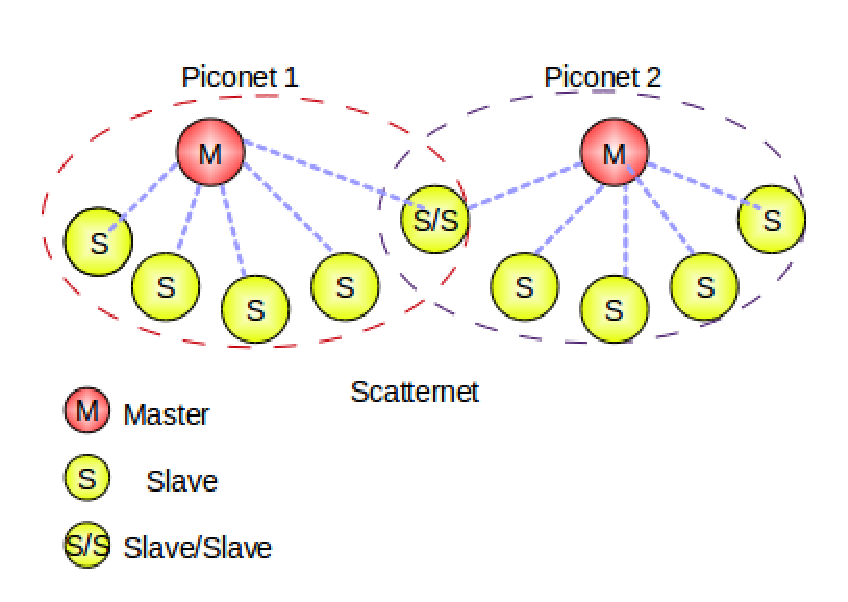
\includegraphics[scale=0.60]{images/scatternet.pdf} 
		\caption{Piconets and Scatternets}\label{fig:scatternet}
	\end{figure}

The piconet/scatternet allows the devices to share the same physical area, allowing the network to make an efficient use of the bandwidth. A Bluetooth system can use up to 79 different frequencies using a frequency hopping (from 2.402 to 2.480 GHz) \cite{bluetoothStack} scheme with a carrier spacing of 1MHz. This allows a bandwidth of 80MHz. Without frequency hopping scheme, every single channel would have a bandwidth of 1MHz at their disposal. With frequency hopping, the sequence will define a logical channel. This allows to have an available bandwidth of 1MHz at any given time, with a maximum of eight devices sharing the bandwidth. This 80 MHz bandwidth can be shared by several different logical channels. Though, this can cause signal collisions when devices in different piconets, on different logical channels have the same hop frequency at a given time. Signal collisions degrade the performance, so we can state that the more piconets we have, the more collisions occur, the lower our total performance will be \cite{introBluetooth}.

	\subsection{Protocol architecture}
The Bluetooth protocol architecture consists of four basic layers: core protocols, cable replacement, telephony control protocols and adopted protocols. Figure \ref{fig:bluetoothStack} shows the architecture of the Bluetooth protocol stack.
	\begin{figure}[ht]
		\centering
		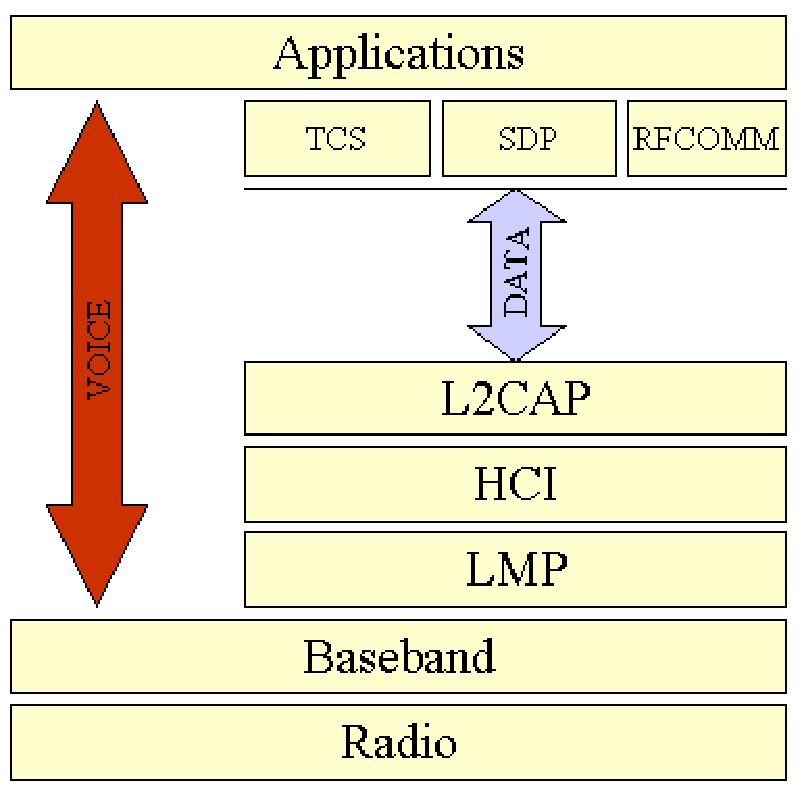
\includegraphics[scale=0.5]{images/bluetoothStack.pdf}
		\caption{Bluetooth protocol stack}\label{fig:bluetoothStack}
	\end{figure}

		\paragraph{Core protocols.}
The core protocol is a five-layer stack. Every layer in the stack has its own responibilites that are mentioned below.

		\begin{itemize}
			\item The \textit{radio} layer is the wireless connection that specifies certain details about the air interface, including frequency, the use of frequency hopping, modulation scheme and transmit power. 
			\item The \textit{baseband} layer is responsible for the packet transmission to the radio layer. As mentioned before this data can contain data or voice packages. For the data packages, asynchronous connectionless (ACL) links are used while voice packages are transmitted with synchronous connection-oriented (SCO) links. The baseband layer maintains both ACL and SCO links. It is important for data packages to be transmitted correctly to maintain data integrity, while it is not a problem in case some voice packages get lost. That is why SCO packages are never retransmitted. If you would retransmit voice packages, every next package would suffer from a time delay restraining us from having real-time communication.
			\item The \textit{Link manager protocol (LMP)} uses the links setup by the baseband and manages the connection between Bluetooth devices. Furthermore, it is responsible for monitoring service quality, security aspects such as device authentication, encryption plus the control and negotiation of baseband packet sizes.
			\item The \textit{Host controller interface (HCI)} is the layer between the hardware and the software. The L2CAP layer and the layers above it are implented in the software while all other layers under the HCI (LMP, baseband, radio) are part of the hardware. The HCI driver acts as a physical bus that connects the hardware with software. It is possible to access the L2CAP layer directly by the application making it easier for application programmers. This makes the HCI, in some cases, an unnecessary component.
			\item The \textit{Logical link control and adaptation protocol (L2CAP)} receives application data and transforms this to the Bluetooth format. Furthermore, Quality of Service (QoS) parameters are exchanged at this layer \cite{bluetoothStack}.
			\item According to \cite{bluetoothStack}, the \textit{Service discovery protocol (SDP)} is not a part of the Core protocols. Though, it contains all the information, services and charasteristics  in order to establish a connection between two or more Bluetooth devices. The LMP uses the SDP's first to find out what services are available from the acces point. Then information from the SDP is obtained by the LMP to create a L2CAP channel.
		\end{itemize}
		
		\paragraph{Cable replacement.}
The RFCOMM seen in figure \ref{fig:bluetoothStack} is the cable replacement protocol. It is a virtual serial port that is designed to replace cable technology. Serial ports are common types of communication interfaces used with computing ang communication devices \cite{introBluetooth}. So with RFCOMM we eliminate the need for serial ports for communication between two devices, assuming both are equiped with a Bluetooth radio. 
EIA-232, once known as RS-232, is a widely used serial port interface standard. The RFCOMM will provide binary data transport and has to emulate EIA-232 control signal to the baseband layer.

		\paragraph{Telephony control protocols.}
Telephony control specifications (binary) or TCS BIN, is a bit-oriented protocol that is necessary to define the call control services in order to establish speech or data calls between the Bluetooth devices.

		\paragraph{Adopted protocols.}
Adopted protocols are protocols developed by other organizations. They are "adopted" into the overall Bluetooth architecture. They are usually standard protocols well known in applications other than Bluetooth. Bluetooth's strategy is to only invent necessary protocols and use existing standard protocols whenever possible. The following standards are the adopted protocols:

	\begin{itemize}
		\item The \textit{PPP}, or point-to-point protocol is as a internet standard protocol for transporting IP datagrams over point-to-point links.
		\item \textit{TCP/UDP/IP}, are the foundation protocols of the TCP/IP protocol suite.
		\item \textit{The object exchange protocol}, or OBEX, is a session level protocol made by the Infrared Data Association (IrDA). It is used for exchaning objects. OBEX comes with quite similar funcionalities as HTTP, but in a simpler way. There is also a model included in OBEX that is used for the representation of objects and operations.
		\item Bluetooth also adopts the wireless application environment \textit{WAE} and the wireless application protocol \textit{WAP} into its architecture.	
	\end{itemize}


\section{Web sockets}
Web sockets are used for fast, real-time communication between a server and a client. The HTTP model, which is also a communication protocol between a server and a client, allowed the client only to request data from the server, while the server was only able to fulfill these requests. Web sockets on the other hand, allow bidirectional communication, or bidi communication, between the server and the client. This means both client and server can request data and also respond to these requests. The main point of web sockets is to have true concurrency and to focus on the optimization of performance when it comes to communication and exchanging data. The web socket protocol that will be discussed is also known as the RFC6455 model \cite{RFC6455}.

	\subsection{Web socket communication}
		\paragraph{Handshake.}
To communicate over web socket, the server and the client first have to connect with each other. The establishment of a web socket connection is done by a web socket handshake. Handshaking is the exchange of information between two devices and the agreement about which protocol will be used to exchange data after the connection is established. A well known example of this is the TCP three-way-handshake. The client sends a synchronization message (SYN) to the server as a request to synchronize with the server. If the server receives this message and allows the client to synchronize with it, it will send a similar SYN message and an acknowledgement message (ACK) to let the client know that it has received the request. When the client receives the SYN-ACK message, it will send an ACK message back to the server to acknowledge that it has received the server's message. The TCP connection is established whenever the server receives the ACK message from the client.\\
The web socket handshake is quite similar. The client sends a handshake request to the server, and the server will respond with a similar handshake request as seen in figure \ref{fig:WebSocketHandshaking}. The desktop, smartphone and tablet in figure \ref{fig:WebSocketHandshaking} represent the clients that are connected to the server. The handshake request from the client-side is shown in listing \ref{lst:clientHandshake}, while the response from the server is shown in listing \ref{lst:serverHandshake}.
	\begin{figure}[ht]
		\centering
		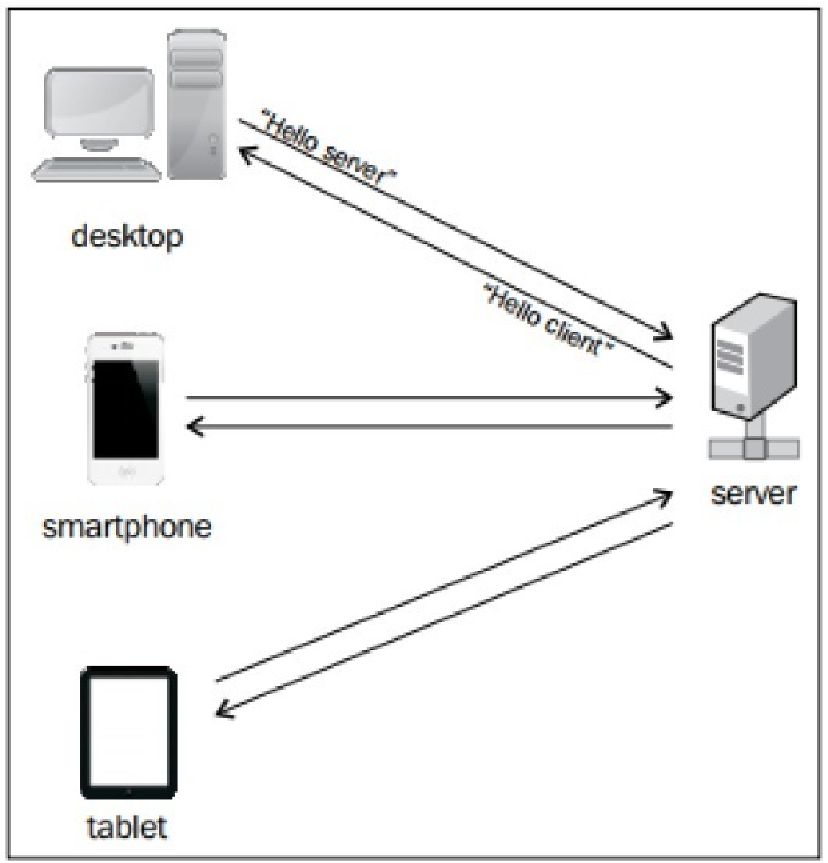
\includegraphics[scale=0.5]{images/server.pdf}
		\caption{Web socket handshaking}\label{fig:WebSocketHandshaking}
	\end{figure}
	\begin{lstlisting}[caption={Client's request for websocket handshake},captionpos=b, label={lst:clientHandshake}, language=c, float=h]
  1| GET /chat HTTP/1.1
  2| Host: example.com:8000
  3| Upgrade: websocket
  4| Connection: Upgrade
  5| Sec-WebSocket-Key: dGhlIHNhbXBsZSBub25jZQ==
  6| Sec-WebSocket-Version: 13
	\end{lstlisting}\\
Listing \ref{lst:clientHandshake}, the handshake request from the client, is a pretty standard HTTP request. It is built with multiple headers, some of which are mandatory for the request to be valid. If one of the headers is not understood, the server will reply with "400 Bad Request" and it will close the socket afterwards. In some cases, it will also give a reason why the handshake failed, although browsers do not display these messages. If there is a problem with version numbers, the server adds a "Sec-WebSocket-Version" header in the HTTP response that contains the version it understands \cite{BadRequest}.
	\begin{lstlisting}[caption={Server's response for websocket handshake},captionpos=b, label={lst:serverHandshake}, language=c, float=h]
  1| HTTP/1.1 101 Switching Protocols
  2| Upgrade: websocket
  3| Connection: Upgrade
  4| Sec-WebSocket-Accept: s3pPLMBiTxaQ9kYGzzhZRbK+xOo=
  5|
	\end{lstlisting}
When the server receives a request handshake from a client with all the necessary headers, it will reply with a HTTP response as shown in listing \ref{lst:serverHandshake}. The "Sec-WebSocket-Accept" header is derived from the "Sec-WebSocket-Key" header from the client's handshake request. To get it, we combine the "Sec-WebSocket-Key" header and "258EAFA5-E914-47DA-95CA-C5AB0DC85B11" together. The second string is "a magic string". A magic string is predefined by the developer in a way where he will never expect this string to come from an external source. When the "Sec-WebSocket-Key" header and the magic string are combined, the SHA-1 hash is taken from the result, and the base64 encoding of the hash is returned \cite{BadRequest}. The SHA-1 is a cryptographic hash function, while base64 is a binary-to-text encoding scheme.

		\paragraph{WebSocket URI's}
WebSocket defines two URI schemes. You can either use ws or the wss scheme. The ws (web socket) is a regular connection similar to http. While wss (web socket secure) is a secured connection similar to https. The schemes are built like the following:\\

\indent	ws-URI = "ws:" "//" host [ ":" port ] path [ "?" query ]\\
\indent	wss-URI = "wss:" "//" host [ ":" port ] path [ "?" query ]\\

The most important components of the ws or wss are the host and its port. The host is determined by the server's IP address, while the port defines which port the server uses for the communication. If there is no specified port, the standard port used for ws is 80, and the standard port used for wss is 443.
		
		\paragraph{Data Frames.}
The main advantage of websockets is bidi communication. So at any point in time, either the client or the server can send a message. Every data frame that is sent from the client to the server, or vice versa, follows the same format as seen in figure \ref{fig:dataFrame}.

	\begin{figure}[ht]
		\centering
		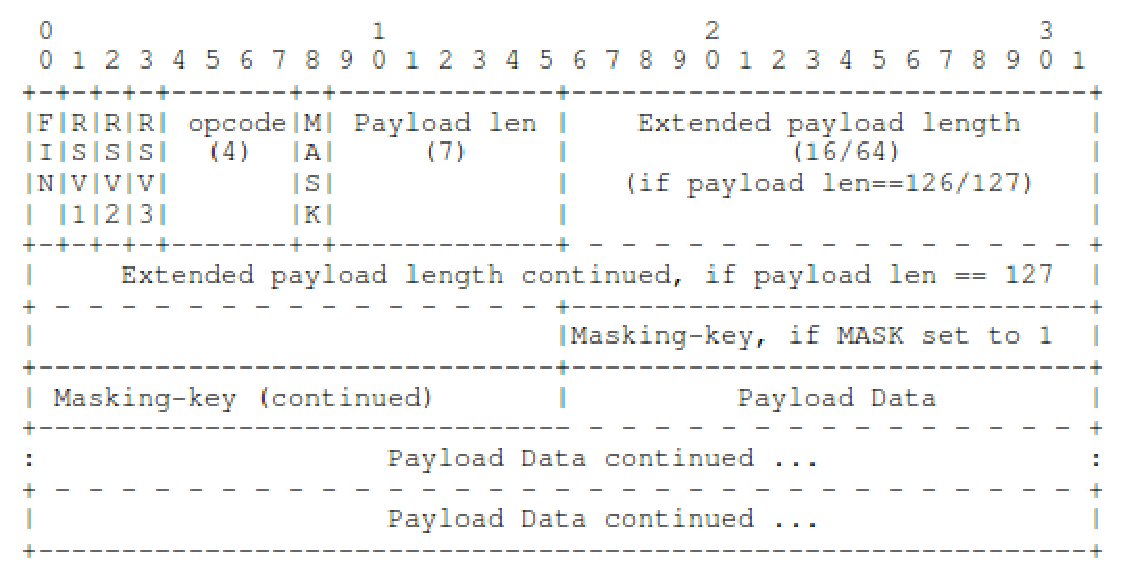
\includegraphics[scale=0.5]{images/WebSocketDataFrame.pdf}
		\caption{Standard WebSocket dataframe format}\label{fig:dataFrame}
	\end{figure}

	\begin{itemize}
		\item {FIN: 1 bit}
	\end{itemize}
Depending on the value of this bit, it either tells the receiving end whether or not this is the final fragment of the message. If the bit equals "0", it is not the last fragment and the receiver will continue listening for more fragments. If the bit equals "1", it means it is the last fragment of the message and the server will consider the message being delivered.
	\begin{itemize}
		\item {RSV1, RSV2, RSV3:  1 bit each}
	\end{itemize}
All of these bits are reserved for websocket extensions. They should be "0" unless the client and server negotiated on whether or not a specific extension requires the use of any of the three bits. If any of these three bits is not zero while the client did not negotiate on any of these bits being non-zero, the receiving end will "fail" the websocket connection.
	\begin{itemize}
		\item {Opcode:  4 bits}
	\end{itemize}
These 4 bits will define how the receiving end should interpret the data. If the receiving end does not understand the opcode it will, as in the previous case, "fail" the websocket connection. The information about the different opcodes is found at \cite{opcode}.
	\begin{itemize}
		\item[] {x0: continuation frame; this frame contains data that should be appended to the previous frame}
		\item[] {x2: binary frame; this frame (and any following) contains binary data}
		\item[] {x3 - x7: non-control reserved frames; these are reserved for possible websocket extensions}
		\item[] {x8: close frame; this frame should end the connection}
		\item[] {x9: ping frame}
		\item[] {xA: pong frame}
		\item[] {xB - xF: control reserved frames}
	\end{itemize}
	\begin{itemize}
		\item {Mask bit: 1 bit}
	\end{itemize}
This bit tells wether or not the frame uses a mask. If this bit is set to "1", a masking key is included in the message.  This masking key is used to unmask the data in the payload. Every frame that is sent from the client to the server must have this bit set to "1".
	\begin{itemize}
		\item {Payload length: 7 bits, 7+16 bits, 7+64bits}
	\end{itemize}
The seven bits determine the length of the payload. If these seven bits equal 126, or "1111110", the actual length is determined by bits 16 to 31 (so 16 extra bits). These are the following 2 bytes. If the seven bits equal 127, or "1111111", the actual length is determined by bits 16 to 79 (so 64 extra bits). These are the following 8 bytes.

	\begin{itemize}
		\item {Masking key: 4 bytes}
	\end{itemize}
As mentioned previously, this field only exists if the mask bit is set to one. All the messages who have this field set to one, are masked by a 32-bit value. If the mask bit is set to zero, there will be no masking key in the first place.

	\begin{itemize}
		\item{Payload data: x+y bytes}
	\end{itemize}
The payload data is the combination of the extension data and the application data. These two are listed below.

	\begin{itemize}
		\item{Extension data: x bytes}
	\end{itemize}
The extension data is non-existent unless it was negotiated on the opening handshake between the server and the client. As mentioned earlier, the RSV1-3 bits are responsible for these extensions. Any extension that has been negotiated by the client and server must have a specified length of the "Extension data". It can also tell the receiving end on how to calculate this length. As said previously, the extension is part of the total payload data.
	
	\begin{itemize}
		\item{Application data: y bytes}
	\end{itemize}
The application data contains the actual data that has be to transmitted. It takes up the remaining space in the frame after any extension data. The application data is, like the extension data, part of the payload data.

	\paragraph{Sending and receiving data.}
In order to send a message as a client, the server must perform the following steps:

	\begin{enumerate}
		\item The receiving end has to make sure the websocket is in an open state. 
		\item last part of web socket that i have to finish......
	\end{enumerate}
		

	%*\subsection{Web socket architecture}
	
	%\begin{figure}[ht]
	%	\centering
	%	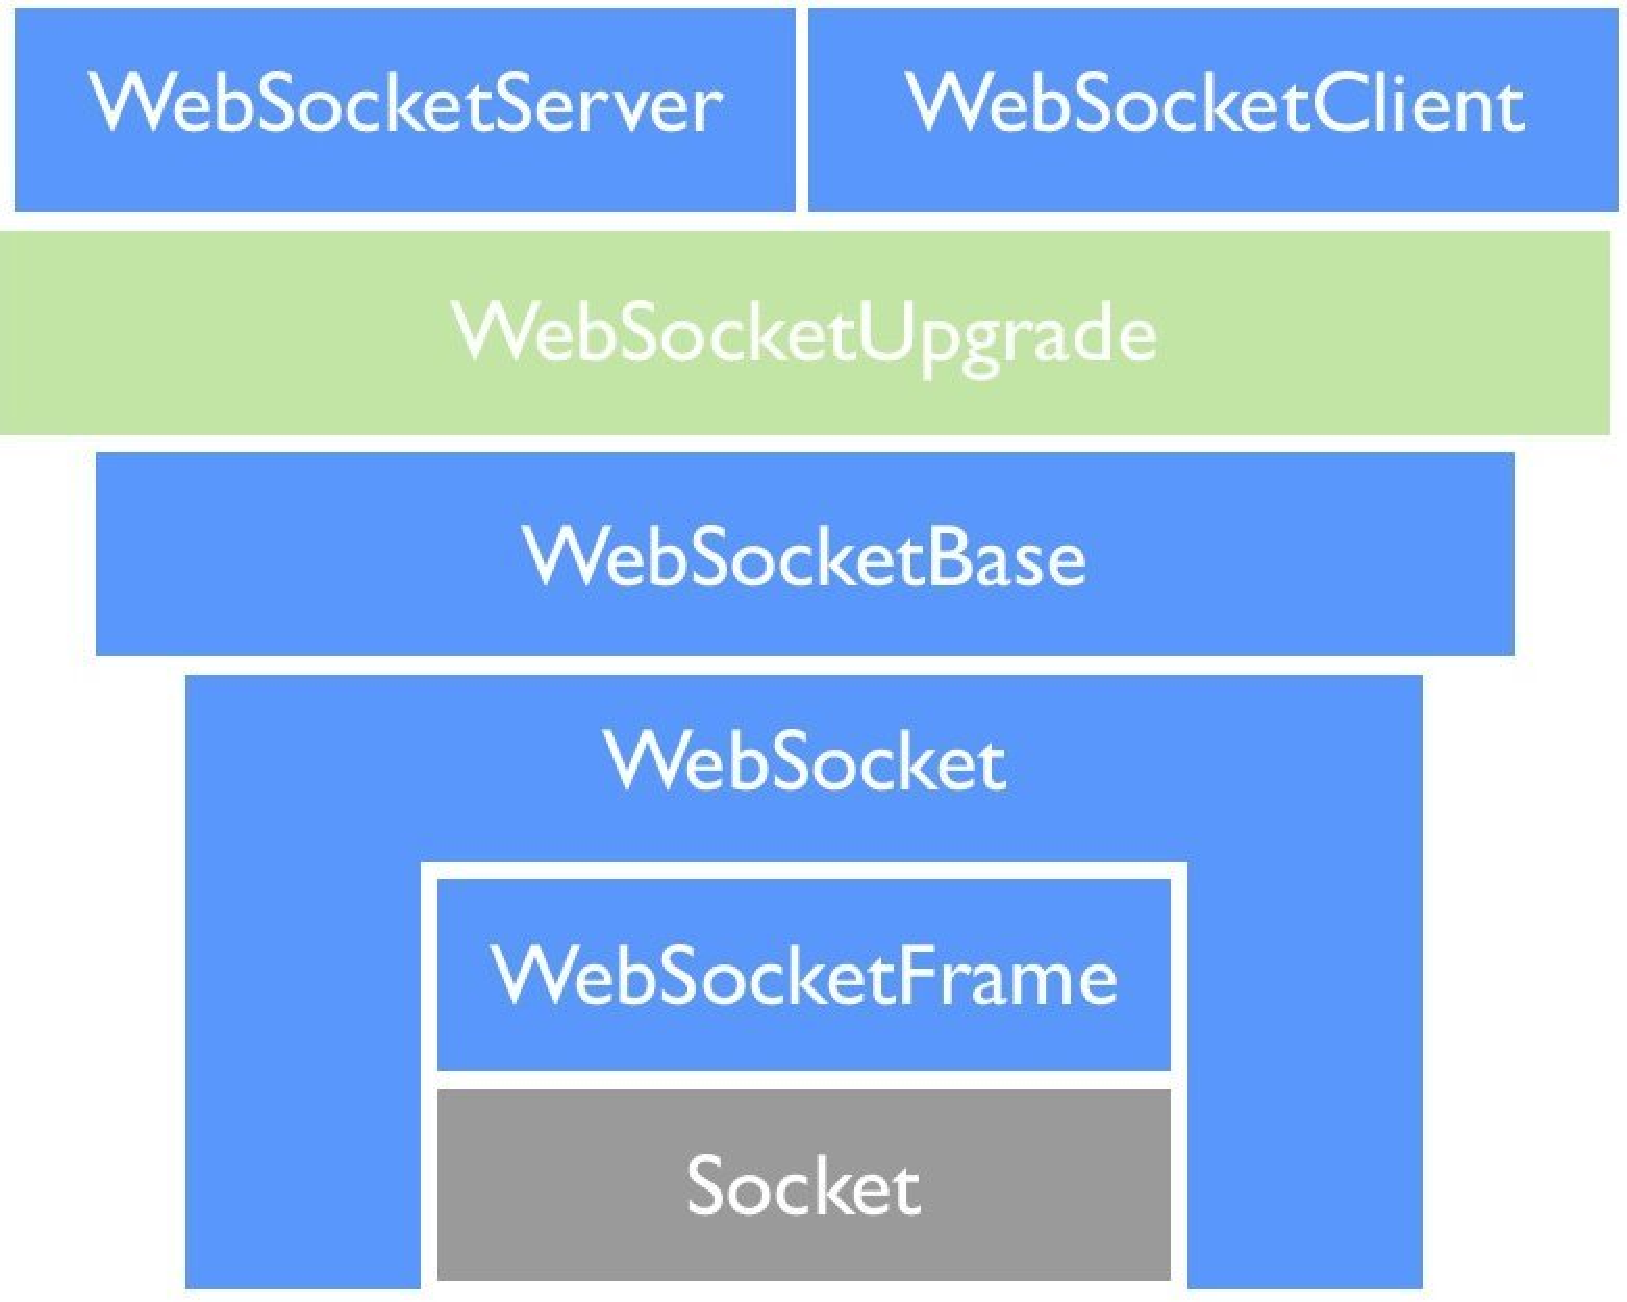
\includegraphics[scale=0.3]{images/websocketsArchitecture.pdf}
	%	\caption{WebSocket architecture}\label{fig:WebSocketArchitecture}
	%\end{figure}
	
	
\section{Communication protocol}
If we want to communicate between the devices, we have to define a set of rules that each one of the devices have to follow. These rules should be made in a way that 100\% of the transmitted data will arrive at the receiving end. For example, if data gets lost through transmission, the device on the receiving end will not receive all the necessary data. This can be prevented by adding some sort of characters that will define what the received message should look like. If the received message looks incorrect, the receiving device has to respond by asking to resend this piece of data. We are trying out two different communication technologies so we have to set up a communication protocol for each one of them since they both have different performance aspects.

	\subsection{Bluetooth protocol}
To define a set of rules we first analyzed how good the Bluetooth transmission is. We did some testing and came to the conclusion that there was quite a lot of data loss. We first tried sending eight characters at once but nearly 80\% of the time there was atleast one of the characters missing. Missing one number would mean that the matrix we need is incorrect and this would lead to an incorrect outcome. We did some further testing and realized it was the best option to send four numbers at a time.
In order to make sure all characters would arrive at the receiving end, we added an extra character ':' at the end of each message. An example of a message would look like this: 4372: .
Now for the communication, we start off by connecting both devices with Bluetooth. As soon as the devices are connected to each other, the SoC will send a message to the Android phone that it is ready to receive the two matrices. This is message 'C' in figure bla




	

\bibliographystyle{IEEEtran}
\bibliography{References}
\end{document}
